

\section{Profiling Tools and Techniques}
\label{prof_tools_techniques}


\begin{frame}
	\frametitle{Profiling Tools and Techniques}
	\begin{itemize}
		\item Bootchart \pause
		\item Bootloader Timestamp \pause
		\item Initcall Debug \pause
	\end{itemize}
\end{frame}

\subsection{Bootchart}

\begin{frame}
\begin{figure}[h]
  \centering
    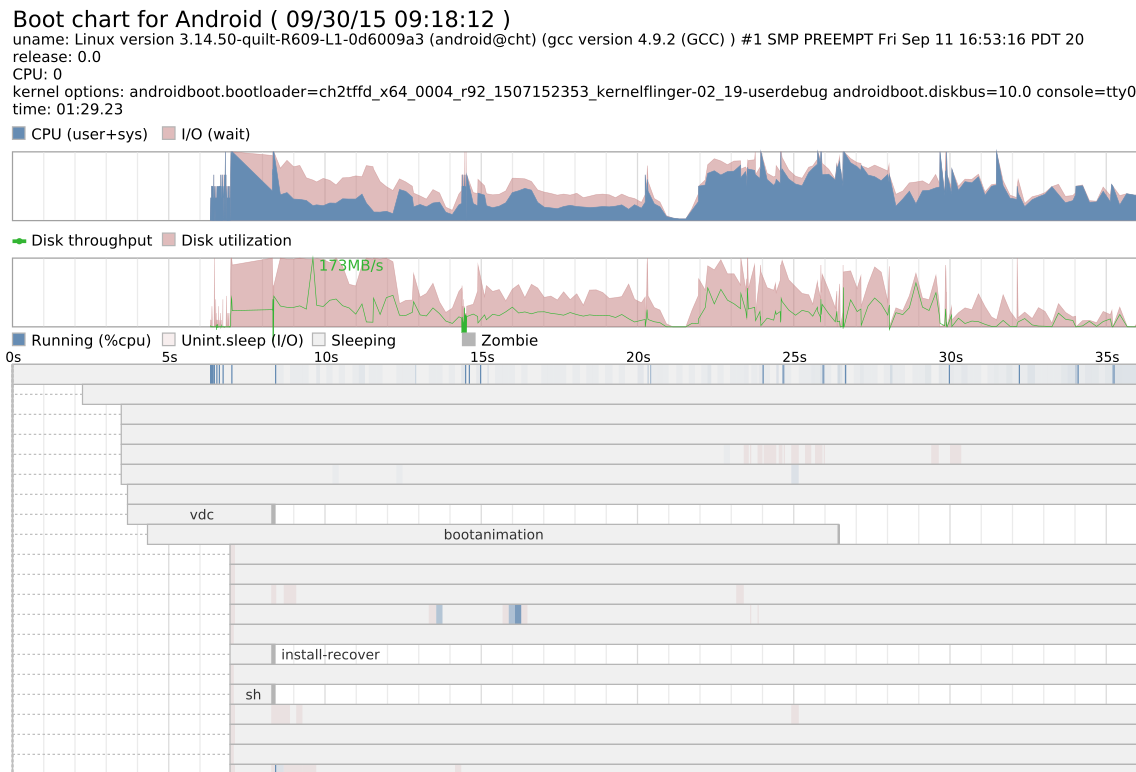
\includegraphics[scale=0.3]{bootchart.png}
    \caption{Bootchart output from Android}
    \label{fig:android_boot}
\end{figure}
\end{frame}

\subsection{Bootloader Timestamps}

\begin{frame}
	\frametitle{Profiling Tools and Techniques}
\begin{enumerate}
	\item Using UEFI {\bf GetTime()} function \pause
	\item Using Host-side serial timestamp \pause
	\item Using {\bf RDTSC} instruction \pause
\end{enumerate}
\end{frame}


\subsection {Initcall Debug}

\begin{frame}[fragile]
	\frametitle{Initcall Debug}
	\begin{itemize}
		\item Kernel command line argument \pause
		\item Trace Driver Initilization function \pause
		\item Measure Time for completion \pause
	\end{itemize}
	\begin{Verbatim}[fontsize=\small]
	dmesg -s 128000 | grep ``initcall`` | \ 
	sed ''s/\(.\)after\(.\)/\2 \1/g'' | sort -n -r
	\end{Verbatim}
\end{frame}


\begin{frame}[fragile]
	\frametitle{Sample output}
	\begin{adjustwidth}{-2em}{-2em}
\begin{Verbatim}[fontsize=\footnotesize]
322342 usecs <7>[ 1.230001] initcall i915_init+0x0/0x74 returned 0
254394 usecs <7>[ 4.872194] initcall ov8858_init_mod+0x0/0x1000 returned 0
220703 usecs <7>[ 0.455998] initcall acpi_init+0x0/0x25e returned 0
214826 usecs <7>[ 1.488846] initcall dwc3_pci_driver_init+0x0/0x1b returned 0
209263 usecs <7>[ 5.364468] initcall atomisp_init+0x0/0xd51 returned 0
199893 usecs <7>[ 0.781643] initcall populate_rootfs+0x0/0xd8 returned 0
133947 usecs <7>[ 2.253326] initcall pmic_ccsm_init+0x0/0x14 returned 0
133379 usecs <7>[ 5.121348] initcall init_lm3554+0x0/0x1000 returned 0
113899 usecs <7>[ 1.890387] initcall intel_pram_init+0x0/0x1d3 returned 0
92015 usecs <7>[  4.975765] initcall init_ov2722+0x0/0x20 returned 0
\end{Verbatim}
	\end{adjustwidth}

\end{frame}

